% !TEX root = ../main.tex
% !TeX spellcheck = fr_FR

\chapter{Expériences automatisées et reproductibles pour \ac{LLN}s} 
\label{makesense}

% \epigraph{It doesn't matter how beautiful your theory is, it doesn't matter how smart you are. 
% If it doesn't agree with experiment, it's wrong.}{Richard Feynman}

\epigraph{Besides black art, there is only automation and mechanization.}{Federico Garcia Lorca}

\minitoc

% Bien qu'étant une contribution importante, le contenu de ce chapitre n'est pas indispensable à la compréhension de la suite de cette thèse.
% Le lecteur désirant se concentrer sur les contributions relatives à la passerelle sans s'attarder sur la méthodologie des expériences pourra passer directement au chapitre suivant.
Ce chapitre présente Makesense, un framework permettant d'obtenir des expériences reproductibles, documentées et automatisables visant les \ac{LLN}s.
L'organisation du chapitre est la suivante:

La section~\ref{makesense:reproductibility} présente la reproductibilité d'expérience et la met en perspective avec la recherche sur les \ac{LLN}s.

La section~\ref{makesense:related} présente comment la documentation et l'automatisation sont faits dans l'état de l'art, comment l'interaction avec les nœuds physiques d'une plateforme est classiquement faite et les limites de chacune de ces approches.

La section~\ref{makesense:makesense} présente Makesense et les choix techniques effectués pour l'utiliser efficacement dans le contexte des \ac{LLN}s.

La section~\ref{makesense:conclusion} conclut ce chapitre en justifiant l'intérêt d'un tel framework pour la communauté scientifique.

\section{Introduction à la recherche reproductible dans les \ac{LLN}s}
\label{makesense:reproductibility}

\subsection{Reproductibilité}

Une expérience est définie comme une série d'actions ayant pour but de tester (confirmer ou infirmer) une hypothèse~\cite{fisher1960design,bachelard1975nouvel}.
Il y a trois éléments impliqués dans ce processus: le \emph{laboratoire} qui correspond à l'environnement (conditions, scénarios, etc.) dans lequel l'expérience se produit, l'\emph{expérimentateur} qui est la personne qui va faire l'expérience et le \emph{dispositif} qui est étudié. 
Si une expérience peut être exécutée dans des laboratoires avec des expérimentateurs et des dispositifs tous différents, mais arriver aux mêmes conclusions alors l'expérience est dite reproductible.

Dans le cas des \ac{LLN}s, une expérience peut consister à tester qu'un système (par exemple un cache) diminue le trafic qu'un \ac{LLN} doit gérer.
Dans ce cas, le laboratoire est l'endroit où cette expérience se produit, l'expérimentateur est l'agent humain ou automatisé effectuant l'expérience et le dispositif est le \ac{LLN} (simulé, émulé ou réel) étudié.

Construire une expérience reproductible est à la base de la méthode scientifique.
Pourtant mettre en place un environnement permettant de construire des expériences reproductibles est souvent perçu comme long et fastidieux.
De plus, la reproductibilité est peu valorisée à court terme aussi bien au moment de juger un article pour le publier dans une revue qu'après sa publication~\cite{fink2013conducting,wilson2014best} et cela malgré son importance fondamentale~\cite{popper-scientificdiscovery}.
Ce paradoxe a été relevé à de nombreuses reprises dans d'autres sciences et existe aussi en informatique \cite{peng2011reproducible}.

Des dépôts de documents scientifiques rendent aujourd'hui possible l'hébergement des fichiers nécessaires au déroulement d'une expérience en plus de la publication en elle-même.
Ainsi réduire la difficulté de mise en place d'expériences reproductibles est le verrou technique principal pour permettre sa diffusion et sa démocratisation.

\subsection{Problématiques expérimentales des \ac{LLN}s} 

Développer une expérience pour \ac{LLN} peut être complexe en raison de la grande hétérogénéité des technologies mises en jeu (systèmes embarqués, transmissions de messages sur réseau, analyse de résultats)~\cite{baronti2007wireless}.
Ainsi des compromis doivent être trouvés entre le degré de réalisme souhaité et le temps de développement nécessaire pour mettre en place une expérience afin d'avoir des résultats pertinents au plus tôt.

\begin{figure}[ht]
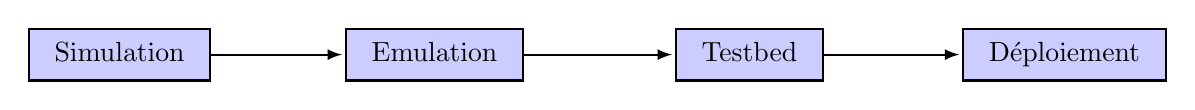
\begin{tikzpicture}[->,>=latex,shorten >=1pt,auto,node distance=3cm,
  thick,main node/.style={fill=blue!20,draw}]

  \node[main node] (sim) at (0,0) {\begin{tabular}{c}Simulation\end{tabular}};
  \node[main node] (emu) at (4,0) {\begin{tabular}{c}Emulation\end{tabular}};
  \node[main node] (iotlab) at (8,0) {\begin{tabular}{c}Testbed\end{tabular}};
  \node[main node] (final) at (12,0) {\begin{tabular}{c}Déploiement\end{tabular}};

  \path
    (sim) edge[] (emu)
    % (emu) edge [bend left=10] node[below] {Modèle} (sim)

    (emu) edge[] (iotlab)
    % (iotlab) edge [bend left=10] node[below] {Prototype} (emu)

    (iotlab) edge[] (final)
    % (final) edge [bend left=10] node[below] {Finalisation} (iotlab)

;
\end{tikzpicture}
\caption{Évolution d'une expérience vers le réalisme}
\label{makesense:fig:workflow}
\end{figure}

La Figure~\ref{makesense:fig:workflow} illustre les différents choix de niveaux d'abstraction de développement pour une expérience portant sur les \ac{LLN}s.
Il existe essentiellement 4 niveaux d'abstraction différents chacun ayant un différent compromis entre réalisme et facilité de développement.

Les simulateurs et émulateurs n'utilisent pas des nœuds physiques et permettent d'avoir dans un programme un fonctionnement modélisé d'un \ac{LLN} afin d'illustrer son fonctionnement aussi rapidement que possible.

Vérifier des résultats de simulations sur des nœuds physiques apporte une confirmation aux résultats trouvés en simulation.
Cependant effectuer des expériences sur un grand nombre de nœuds requiert de disposer physiquement de ces nœuds.
Il peut être coûteux pour un laboratoire d'investir pour acheter, mettre en place et maintenir tous les nœuds requis pour une expérience donnée.
Ainsi des plateformes publiques (``testbeds'' en anglais) sont apparus afin de mutualiser un grand nombre de nœuds physiques entre plusieurs équipes de recherche~\cite{doddavenkatappa2012indriya, fleury2015fit}.
Ces plateformes mettent à la disposition de leurs utilisateurs des nœuds physiques avec des architectures matérielles variées sur lesquels un utilisateur déploie son système.
Elles offrent des traces détaillées de l'expérience et permettent de déployer sur des nœuds représentatifs d'un capteur un code spécifique et de mesurer l'évolution de ce nœud au cours du temps~\cite{fleury2015fit}.

Les sous-sections suivantes exposent plus en détail les différents compromis de chaque niveau et la difficulté de porter les développements faits à un niveau donné vers un niveau plus réaliste.

\subsubsection{Expérience sur simulateur}
\label{makesense:simulation}

Un simulateur permet d'avoir une modélisation du \ac{LLN} sous la forme d'un programme qui une fois exécuté renvoie des résultats~\cite{sobeih2006j,abdeddaim2011implementation}.

L'atout d'un simulateur réside dans son environnement qui est totalement contrôlé, détaillé et sur la capacité de simuler des scénarios avec un grand nombre de nœuds sur des temps longs avec des temps courts de simulation~\cite{jevtic2009evaluation}.
Si les graines des générateurs de nombres aléatoires sont fixées, alors on a une reproductibilité complète de l'expérience si on ré-exécute le même programme avec les mêmes entrées deux fois de suite.
En outre, le simulateur étant un système isolé, corriger le système et tester une nouvelle idée est relativement facile.

Cependant, les simulateurs font un certain nombre d'approximations sur le médium de transmission et plus généralement sur le fonctionnement des nœuds, la dérive des horloges, l'usure des composants et les pannes éventuelles.
Ainsi les simulations ne correspondent pas fidèlement à un déploiement sur nœuds réels et des problèmes non prévus peuvent subvenir lorsqu'un déploiement réel se produit.

\subsubsection{Expérience sur émulateur}
\label{makesense:emulation}

Un émulateur permet de substituer une architecture matérielle physique par un logiciel.
Les émulateurs sont activement utilisés afin de permettre un développement logiciel rapide qui ne nécessite pas d'installer un code sur un nœud physique à chaque changement~\cite{cooja}.

Ainsi dans le cas d'une simulation, au lieu d'utiliser un programme ad hoc le simulateur utilise un émulateur d'architecture matérielle afin de disposer d'informations plus réalistes sur le fonctionnement d'un nœud comme des visualisations du cycle de veille des nœuds, de la consommation énergétique estimée de chaque nœud et de pouvoir inspecter le code s’exécutant sur un nœud durant une simulation.
Émuler permet de tester un code réel, tandis que simuler oblige à utiliser une abstraction du code exécuté.

Cependant, un émulateur est soumis aux mêmes limitations qu'un simulateur, toutes les interactions (transmission, dérive d'horloge) sont modélisées par des logiciels et sont donc d'un réalisme limité.

\subsubsection{Expérience sur plateforme}
\label{makesense:testbeds}

L'objectif des déploiements sur plateforme est de fournir des nœuds physiques réels aux expérimentateurs afin d'exécuter des expériences dans des conditions plus réalistes que celle d'un simulateur ou d'un émulateur.

L'utilisation des plateformes est répandue en recherche et de nombreux travaux s'appuient sur ces plateformes pour effectuer des expériences~\cite{theoleyremesures,handziski2006twist}.

Cependant, effectuer une expérience sur plateforme présente des différences de fond par rapport aux expériences sur simulateur et émulateur.
Le temps ne pouvant être accéléré comme sur un simulateur, des expériences longues sont nécessaires pour tester la fiabilité sur de grandes périodes de temps.
Puisque les nœuds sont réels, ils peuvent tomber en panne et avoir des avaries, ainsi, il est impossible de garantir de manière systématique et déterministe, que deux expériences donneront exactement les mêmes résultats. 

Dans le cas de plateformes mutualisées et distantes, il est nécessaire de partager les réservations des nœuds ainsi que de communiquer avec cette plateforme via des interfaces spécifiques ce qui rajoute un niveau de complexité à l'expérience.
Enfin, les déploiements sur ces plateformes se font le plus souvent sur des nœuds à l'intérieur de bâtiment, statiques dans l'espace, dans des environnements contrôlés et offrant peu de variabilité.
Ainsi, il n'est pas toujours possible de contrôler l'environnement radio, la position des nœuds et l'atténuation des signaux entre les différents nœuds. 

\subsubsection{Expérience en déploiement réel}
\label{makesense:real_deployment}

Déployer une expérience sur nœuds réels permet d'avoir un système dans des conditions aussi réalistes et proches que possible que celles dites de ``production'' d'un système finalisé.

Le réalisme dans ce cas est très proche des conditions réelles d'un \ac{LLN} déployé dans son environnement cible.
Cette phase qui est généralement faite en phase de finalisation est plus coûteuse car il faut disposer des nœuds physiques, les installer dans une zone potentiellement large et subir les conditions logistiques de déploiement~\cite{werner2006deploying}.
Dans ces conditions, modifier les nœuds peut être complexe si l'environnement est hostile ou si les nœuds ne peuvent pas être mis à jour facilement à distance.

\subsubsection{Transitions entre niveaux}
\label{makesense:transition}

L'objectif d'une expérience est de se rapprocher autant que possible de la réalité afin de permettre de modéliser des problèmes et d'y apporter des solutions.
Cette progression vers le réalisme peut être accélérée par la réutilisation des systèmes développés lors d'étapes préalables.

Passer de l'étape de simulation à l'émulation permet de gagner en réalisme et de modéliser plus finement un \ac{LLN} car une partie des contraintes mémoires des architectures matérielles des nœuds sont prises en compte grâce à l'émulateur.
L'analyse des données et leur visualisation peuvent être conservées, car une partie des sorties de l'expérience (par exemple les logs séries) peuvent être au même format et analysées de la même façon.

Le passage de l'émulation à la plateforme permet de gagner en réalisme, car les contraintes des nœuds physiques apparaissent.
Les images binaires produites lors du prototypage avec un émulateur peuvent être conservées, ainsi il n'est pas nécessaire de les réécrire.
De plus, le code écrit pour analyser les résultats peut être également conservé, car les sorties séries peuvent être au même format.

Enfin, le passage de la plateforme au déploiement réel met en jeu des contraintes qui sont spécifiques à un déploiement donné et à sa finalisation, ainsi cette difficulté souvent logistique ne peut être évitée et dépend de chaque contexte.
Cependant le binaire faisant fonctionner les nœuds et l'analyse des résultats conçue précédemment peuvent être conservés.

On peut observer que la progression vers le réalisme est un processus itératif et qu'une partie des développements peuvent être conservés d'un niveau à l'autre afin d'économiser les coûts de mise en place.
Ainsi un framework permettant de documenter, d'automatiser et de réutiliser autant de fonctionnalités que possible entre les différents niveaux permet aux utilisateurs de se concentrer sur les verrous technologiques propres à chaque niveau au lieu de ré-implémenter l'ensemble de leur développement à chaque fois. 

\section{État de l'art sur les outils de gestion d'expériences}
\label{makesense:related}

Gérer une expérience sur des nœuds physiques ou émulés met en jeu de nombreuses étapes comme la préparation des nœuds, l'exécution et le traitement des données.
L'intégration de toutes ces étapes est longue et fastidieuse ainsi il est nécessaire de la documenter et lorsque cela est possible de l'automatiser. 

\subsection{Documentation}

Les logiciels et plateformes utilisés par les \ac{LLN}s sont relativement nouveaux, ainsi, il est particulièrement important que leur documentation soit aussi claire et tenue à jour que possible afin de diffuser efficacement leur usage.
Cette documentation est actuellement essentiellement fournie par des didacticiels ad hoc et des wikis qui sont édités par la communauté des utilisateurs.
C'est notamment le cas des plateformes Indriya et IoT-lab~\cite{fleury2015fit,doddavenkatappa2011indriya} et des systèmes d'exploitation usuels tels que Contiki~\cite{dunkels2004contiki}, OpenWSN~\cite{watteyne2012openwsn} ou encore RIOT~\cite{baccelli2013riot}.
Cette approche est choisie, car elle est facile à mettre en place et permet de rapidement partager une expérience avec les utilisateurs, mais a le défaut de pouvoir devenir obsolète si elle n'est pas tenue à jour.

Une autre approche consiste à documenter un projet de manière systématique par l'utilisation d'un logiciel de documentation comme Doxygen~\cite{van2004doxygen} ou Sphinx~\cite{brandl2010sphinx}.
Cependant cette approche repose sur une idée de projet unique et cohérent, or les expériences sur les \ac{LLN}s mettent en jeu de très nombreux sous-projets hétérogènes dans des langages parfois différents rendant cette approche peu efficace.

Enfin, une approche alternative à la documentation consiste à intégrer du code exécutable dans le même document qui est utilisé pour décrire une expérience.
Ces documents enrichis sont souvent désignés par le terme de \emph{notebook} et sont couramment utilisés dans certaines communautés scientifiques et pédagogiques~\cite{young2003science,shen2014interactive}.
Cependant l'utilisation de ces notebooks est encore restreinte dans la communauté de recherche sur les \ac{LLN}s.

\subsection{Automatisation}
\label{makesense:related_automatisation}

Automatiser une expérience permet de la rendre reproductible, documentée et de la partager plus facilement, car toutes les étapes requises sont décrites dans le programme qui l'automatise~\cite{lee1992tools, king2009automation}.
De plus, l'automatisation d'un système permet de fournir des résultats cohérents d'une exécution d'expérience à l'autre et d'accélérer la prise en main d'un débutant, car toutes les étapes requises sont spécifiées.
En outre, corriger une erreur dans un procédé automatisé permet de l'éviter définitivement alors qu'une correction manuelle appliquée de manière ad hoc doit être effectuée de nouveau lorsque le contexte de l'expérience change.

Afin de décrire les dépendances entre les différentes étapes de l'expérience~\footnote{Par exemple: compiler les nœuds avant de les émuler.}, des outils génériques tels que \texttt{make} sont généralement utilisés pour garantir que les dépendances d'une étape donnée de l'expérience sont à jour~\cite{feldman1979make}.
Cependant, les vérifications préalables au lancement des étapes telles que les dépendances logicielles et matérielles sont rarement documentées ou testées lors de leur automatisation.
Or, ne pas tenir compte de ces différentes dépendances peut provoquer des erreurs subtiles à détecter notamment dans des logiciels en développement actif comme les systèmes d'exploitation des nœuds capteurs d'un \ac{LLN}.

\subsection{Déploiement d'expérience sur nœuds réels}

Un testbed met en jeu de multiples ressources pour des utilisateurs multiples, ainsi la gestion des ressources disponibles et leur réservation est une question fondamentale pour ces plateformes.
L'interface avec les testbeds est une question étudiée et de nombreux outils sont disponibles dans l'état de l'art pour s'interfacer avec eux aussi efficacement que possible~\cite{buchert2015survey}. 
Certains testbeds utilisent des frameworks spécifiques comme \ac{OMF} et son langage de description d'expériences \ac{OEDL} qui peuvent être utilisés pour décrire une expérience et déclencher des actions en fonction d’événements~\cite{rakotoarivelo2010omf}.
Cependant cette approche est coûteuse en temps, car elle requiert d'apprendre un \ac{DSL} qui repose sur un formalisme fixe et qui ne peut pas être réutilisé dans d'autres contextes.
Ainsi des approches plus génériques et indépendantes d'un langage donné sont plus adaptées pour favoriser la diffusion d'une expérience par exemple par l'utilisation d'une \ac{API}.

De plus, les frameworks permettant d'utiliser des testbeds disponibles dans la littérature ne proposent des abstractions que pour la réservation et le lancement d'expériences~\cite{auge2014tools,baron2012towards}.
Les interfaces proposées ne gèrent pas par exemple les processus et leur relance qui doivent être gérés par l'utilisateur.
Ainsi il est nécessaire pour un utilisateur de surveiller l'évolution d'une expérience pour réagir aux pannes éventuelles.
De plus, pour un utilisateur débutant, les multiples erreurs pouvant survenir sont parfois difficiles à interpréter quand peu d'informations sont disponibles pour aider.

\subsection*{Conclusion intermédiaire}

Comme vu dans cette section, l'état de l'art offre des solutions pour chacun des problèmes individuellement cependant leur intégration au sein d'un seul framework cohérent est encore manquant.

Les descriptions de protocoles expérimentaux peuvent être enrichies via un mécanisme de notebook pour fournir à la fois une description et code au sein d'un même fichier.

L'automatisation est nécessaire pour garantir la consistance et la rapidité de mise en place, mais doit être couplée à la vérification des dépendances et intégrée avec la documentation afin de garantir que le code d'une expérience est exécuté dans un contexte défini et que toutes les dépendances sont satisfaites.

Enfin, l'utilisation des testbeds est utile pour avoir des expériences sur nœuds physiques et il faut privilégier leur intégration au sein de mécanismes généraux comme des \ac{API} afin d'éviter des \ac{DSL} qui forcent l'utilisation d'un formalisme spécifique.

\section{Makesense}
\label{makesense:makesense}

Makesense est un framework produit dans le cadre de cette thèse permettant d'obtenir la \emph{documentation}, l'\emph{automatisation} et la \emph{reproductibilité} d'une expérience.
Ce framework vise à réduire le temps nécessaire pour mettre en place une expérience reproductible en intégrant les différentes étapes d'une expérience dans un seul document enrichi afin d'exécuter une expérience aussi bien sur des nœuds simulés, émulés ou réels.
Makesense intègre plusieurs outils afin d'aboutir à cet objectif.

\paragraph{Utilisation d'un notebook pour contenir la documentation et le code d'une expérience}

Makesense utilise un notebook pour contenir à la fois la documentation d'une expérience et le code permettant de l'exécuter.
L'apport de fond d'un notebook se situe dans la juxtaposition de la documentation enrichie et du contexte d'exécution commun à l'ensemble du notebook.
La description d'une expérience dans un notebook est présentée de la même façon que dans un didacticiel, des étapes se suivent dans un ordre précis pour aboutir à un résultat.
Chaque étape peut être rejouée indépendamment, ainsi le coût pour rejouer une étape se limite a l'étape elle-même et pas à ses dépendances qui sont gardées en mémoire.

\paragraph{Utilisation d'un langage et d'un contexte commun}

Utiliser des outils hétérogènes et incapables de communiquer efficacement entre eux augmente la charge de développement et le temps requis pour intégrer ces différents composants~\cite{stanisic2015effective}.
Ainsi Makesense utilise un seul langage et partage un contexte d'exécution entre toutes les étapes afin de simplifier la compréhension d'une expérience et le partage des données.

\paragraph{Utilisation d'outils généraux et communs à plusieurs champs de recherche}

Développer un outil spécifique aux \ac{LLN}s limiterait d'emblée sa portée.
En outre, les processus de gestion d'expériences ont de nombreuses similarités avec des approches génériques de développement logiciel.
Makesense utilise des bibliothèques logicielles scientifiques et généralistes largement diffusées pour effectuer une expérience.
Ce choix permet d'éviter l'obsolescence des dépendances, car elles reposent sur des communautés actives et visent à offrir un pont entre les communautés scientifiques et celles liées au développement logiciel.

\paragraph{Approvisionnement d'expérience par l'utilisation de gabarit}

Les expériences sur les \ac{LLN}s mettent en jeu de nombreux fichiers (code source des nœuds, configuration d'un simulateur, etc.) qui peuvent être réutilisables d'une expérience à l'autre, notamment dans les cas de campagnes d'expériences.
Makesense génère ces fichiers de manière expressive en utilisant des gabarits de fichiers pour générer dynamiquement l'ensemble des fichiers nécessaires à une expérience donnée.
Ainsi une campagne d'expérience composée d'expériences paramétrables peut être conçue rapidement à partir des gabarits et des paramètres spécifiques de cette expérience.

\paragraph{Réutilisation des processus d'exploitation sur différents niveaux d'abstraction}

Une expérience qu'elle se passe sur nœuds simulés, émulés ou physiques conserve d'un niveau d'abstraction à l'autre des processus et des fonctions communes (par exemple l'analyse des données et leur mise en forme).

Makesense permet de documenter et d'automatiser ces processus communs afin de pouvoir les réutiliser autant que faire se peut d'un niveau d'abstraction à l'autre.
Ainsi les transitions entre les différents niveaux sont plus rapides, car les traitements communs sont conservés et peuvent être appliqués en séquence.

\paragraph{Utilisation d'outils de gestion de révisions et d'intégration continue}

Une expérience évolue au cours du temps ainsi il est essentiel de garder en mémoire son évolution et de tester en permanence que les révisions apportées ne cassent pas les résultats précédemment obtenus et que les dépendances sont satisfaites.
Ainsi Makesense utilise un gestionnaire de révision et un service d'intégration continue afin de conserver toute l'évolution du développement d'une expérience et garantir que chaque nouvelle révision d'une expérience n'introduit pas d'erreurs.

\paragraph{Licence et démonstration}

Afin de favoriser son utilisation, Makesense est disponible sous licence Apache sur Github~\footnote{\href{https://github.com/sieben/makesense}{https://github.com/sieben/makesense}} et une démonstration du déroulement d'une expérience est également disponible~\footnote{\href{https://travis-ci.org/sieben/makesense}{https://travis-ci.org/sieben/makesense}}.

\subsection{Présentation d'une expérience typique sur les \ac{LLN}s}

Une expérience portant sur un \ac{LLN} commence le plus souvent par la génération des différents composants nécessaires à sa mise en place: binaire faisant fonctionner les nœuds, préparation et configuration des outils annexes (émulateurs, simulateurs, etc.).
Lorsque ces fichiers sont prêts, ils sont placés sur les machines adéquates: flashage de nœuds physiques, déplacement du programme de simulation vers un nœud de calcul, etc.
Puis l'expérience est lancée, plusieurs processus concurrents sont mis en œuvre pour produire des résultats bruts: démarrage des nœuds physiques, lancement d'un simulateur, collecte des résultats, injection de trafic, etc.
Lorsque l'expérience est terminée, les traces physiques sont analysées pour fournir des résultats quantitatifs et qualitatifs au sujet de l'expérience.

Toutes ces étapes mettent en jeu un grand nombre de technologies hétérogènes et sont donc difficiles à maintenir et documenter efficacement.

Le but de Makesense est de documenter, automatiser et rendre reproduire des expériences scientifiques et vise tout particulièrement les expériences sur les \ac{LLN}s.
Les sous-sections suivantes décrivent comment Makesense apporte une solution aux problématiques préalablement énoncées.

\subsection{Documentation d'une expérience}

Une expérience sur un \ac{LLN} intègre de nombreuses étapes comme la construction des images binaires qui vont être flashées, le lancement des processus, le traitement des données, etc.
Des erreurs peuvent arriver à chaque étape, ainsi leur intégration est coûteuse notamment dans le cas où l'expérimentateur a peu d'expérience au sujet des \ac{LLN}s et des logiciels mis en jeu.

Une approche classique de la documentation d'une expérience consiste à avoir la documentation, le code et les résultats obtenus dans des fichiers distincts.
Cette approche n'offre aucune garantie de filiation entre la documentation, le code et les résultats obtenus notamment dans le cas où la documentation et le code sont encore activement édités.
De plus, dans le cas où il ne s'agit que d'un seul code monolithique, il est nécessaire de le ré-exécuter entièrement pour avoir ses résultats ceci peut s'avérer coûteux dans le cas où des traitements longs sont ré-exécutés inutilement.

Makesense documente ces étapes, en utilisant des notebook afin d'avoir d'un seul référentiel pour le code et la documentation que l'expérience se passe sur émulateur ou sur testbed.

\subsubsection{Introduction sur les notebooks}

Un notebook est un document interactif qui permet de ré-exécuter simplement toutes les étapes d'une expérience afin d'obtenir ses résultats dynamiquement. 
Il est composé d'un noyau effectuant les calculs et de cellules de texte enrichies pouvant être affichées avec une mise en page avancée.

L'annotation et la modification des textes en marge des résultats permettent d'avoir une façon beaucoup plus lisible de partager des résultats et de savoir comment ils ont été obtenus.
En outre, modifier la documentation du processus expérimental est beaucoup plus naturel, car elle se trouve à côté du code permettant de l'obtenir et au sein du même document.

\begin{figure}[ht]
  \centering
  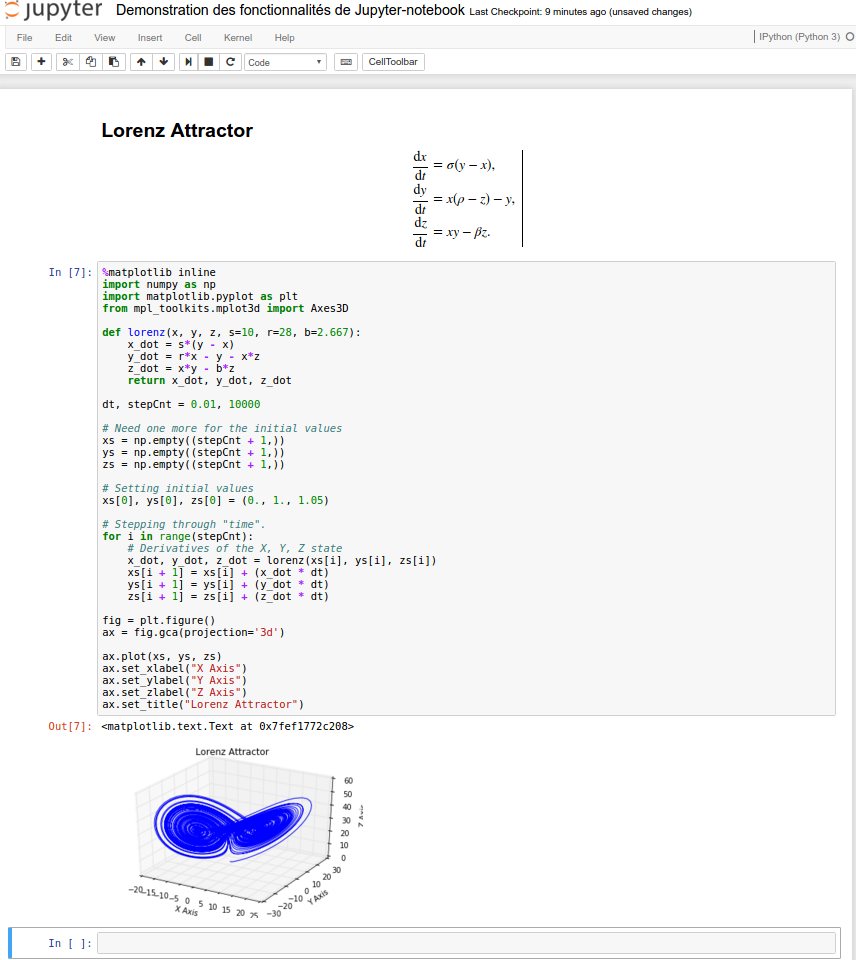
\includegraphics[width=.8\textwidth]{img/jupyter_demo2.png}
  \caption{Capture d'écran d'un notebook ouvert fonctionnant en local et consulté par interface web}
  \label{makesense:fig:demo}
\end{figure}

Un notebook, une fois lancé, peut être vu et utilisé via une interface graphique comme montré sur la Figure~\ref{makesense:fig:demo} qui met en jeu une interface web.
Cette figure met en jeu quatre cellules, la première représente un rendu de texte enrichi avec un titre mis en gras et des formules \LaTeX{} rendues et centrées.
Lorsqu'une cellule de texte est rendue, le texte et les formules mathématiques au format \LaTeX{} ou Markdown contenus  dans cette cellule sont rendus à l'utilisateur permettant d'avoir une mise en page avec des listes, des sections, des images et des formules mathématiques.

La seconde cellule est une cellule de code elle contient du code et des ``built-in magic command'' introduites par le signe \% au début de la cellule et servant à modifier dynamiquement le comportement du notebook.
Lorsqu'une cellule de code est rendue, le code est exécuté dans le noyau qui est un contexte commun pour toutes les autres cellules de code du notebook.
De plus, les cellules de code peuvent être ré-exécutées indépendamment les unes des autres permettant par exemple de séparer les calculs longs et coûteux des calculs plus courts d'exploration ou de visualisation de données.

Enfin, la troisième cellule montre le résultat de l'exécution du code contenu dans la seconde cellule sous forme graphique.
La quatrième cellule est une cellule de code disponible pour être éditée et exécutée de manière interactive.

L'utilisation des notebooks dans les logiciels scientifiques est ancienne et cette technologie est devenue suffisamment mature pour être utilisée aussi bien en recherche qu'en enseignement~\cite{gray1991exploring,young2003science,stevens2013automated,perez2013open}.

Parmi l'ensemble des notebooks libres disponibles, on peut citer Wakari~\cite{tsaftaris2014scientist}, Sage~\cite{stein2008sage}, Apache Zepplin~\cite{manivannan2015scala} ou encore IPython~\cite{PER-GRA:2007}.

Makesense intègre dans un notebook l'ensemble des traitements, paramètres, fonctions et la documentation du protocole expérimental d'une expérience sur les \ac{LLN}s.
Makesense peut fonctionner avec plusieurs formats de notebook différents tant qu'ils supportent certaines fonctionnalités.

Jupyter~\cite{poweredbyjupyter} est un projet proposant une suite d'outils libres pour l'informatique interactive et parallèle scientifique.
Ce projet est une évolution du projet IPython~\cite{PER-GRA:2007} qui a été étendu pour donner le projet Jupyter.
Le Jupyter Notebook est le format de notebook fournit par le projet Jupyter combinant code, texte, images, expressions mathématiques et des fonctions interactives au sein d'un même document qui est encodé dans un format texte documenté~\cite{notebookformat}.
Ces notebooks peuvent être lancés dans des interfaces graphiques ou web qui offrent un rendu graphique et un contexte d'exécution commun par l'utilisation d'un noyau.
Jupyter dispose d'une communauté d'utilisateurs et de développeurs large et dynamique ainsi que de nombreux ouvrages documentant son fonctionnement~\cite{mckinney2012python}.

Les paragraphes suivants détaillent les différents critères et justifient pourquoi Makesense utilise dans cette thèse la plateforme Jupyter et son format de notebook afin de documenter et effectuer des expériences.

\subsubsection{Propriétés recherchées pour un notebook}
\label{makesense:justification_notebook}

\paragraph{Format texte et ouvert}

Reproduire une expérience doit avoir aussi peu de barrières que possible, or acheter une licence ou un abonnement pour utiliser un logiciel propriétaire représente une barrière non négligeable.
Ainsi seuls les formats ouverts et pouvant être utilisés par des solutions libres sont pertinents pour un notebook visant à être utilisé par un public large.

Utiliser un format texte permet en outre de visualiser facilement les différences entre deux versions d'un même notebook par des outils de comparaisons de documents textes classiques ce qui permet de faciliter l'acceptation des contributions extérieures.
De plus, la gestion des révisions est nécessaire pour la mise en place d'une intégration continue efficace qui sera introduite dans la section~\ref{makesense:ci}.

Jupyter Notebook utilise un format texte ouvert et documenté sous la forme d'un \ac{JSON}~\cite{notebookformat} et répond donc à ce besoin fonctionnel.

\paragraph{Flexibilité dans le choix du langage de programmation}

Les préférences de langage de programmation peuvent varier en fonction d'une expérience et des préférences d'un utilisateur.
La notion de notebook est indépendante du langage qu'elle utilise, car c'est avant tout un format contenant du texte enrichi et de la mise en page de cellules.
Ainsi un notebook idéal doit être indépendant d'un langage de programmation donné pour laisser autant de flexibilité que possible à un utilisateur.

Le format de notebook de Jupyter Notebook est découplé de son noyau d'exécution, ainsi il existe plus d'une soixantaine de noyaux différents, écrits dans plusieurs langages de programmation~\cite{poweredbyjupyter}.
Les critères de choix d'un moteur sont relatifs à la disponibilité des bibliothèques logicielles, la stabilité du moteur et les propriétés du langage.

Afin de bénéficier de la plus grande stabilité et d'une large gamme de bibliothèques logicielles scientifiques, Makesense utilise \texttt{ipykernel} qui est le noyau historique de référence de Jupyter codé en Python.
De plus, l'utilisation de Python permet d'interfacer facilement Makesense avec la plateforme IoT-lab (\ref{automation:deploy_execute_move}) par l'utilisation de la bibliothèque officielle d'IoT-lab qui est codée en Python.

\paragraph{Support d'exports et de rendu}

Un notebook utilisé par Makesense doit pouvoir répondre à deux besoins relatifs au partage et l'export d'une expérience afin de pouvoir couvrir un large éventail d'utilisation et être flexible sur les préférences de leurs différents utilisateurs.

Le premier consiste à pouvoir être exportable vers des fichiers statiques (\ac{PDF}, page web, etc.) afin que les résultats d'une expérience puissent être partagés sans nécessiter une installation de dépendances et l'exécution des cellules.

Jupyter-notebook dispose d'un grand nombre d'exports et un rendu automatique des notebooks est supporté par plusieurs plateformes en ligne comme Github~\footnote{\href{https://github.com/sieben/makesense/blob/master/demo.ipynb}{https://github.com/sieben/makesense/blob/master/demo.ipynb}} et nbviewer~\footnote{\href{http://nbviewer.jupyter.org/}{http://nbviewer.jupyter.org}}.
Ainsi un notebook peut être rendu directement sur la plateforme Github pour avoir un rendu similaire à celui de la Figure~\ref{makesense:fig:demo} en ligne et sans installation.
Le rendu sur ces plateformes est fait sur une page web statique pouvant être imprimée ou partagée avec des relecteurs.

Le second besoin consiste à pouvoir extraire les cellules de code vers un programme exécutant l'ensemble de l'expérience.
Cette approche est pertinente pour disposer d'un programme pouvant ré-exécuter l'expérience et produire ses résultats et où le rendu du texte n'est pas souhaité.

Jupyter-notebook supporte ces deux types d'exports et permet ainsi à Makesense de répondre à ce besoin fonctionnel.

\subsection{Automatisation d'une expérience}
\label{makesense:auto}

Automatiser les tâches d'un processus est essentiel pour s'assurer qu'aucune étape n'a été oubliée et qu'elles sont toutes explicitées. 
Dans le cas de développement d'expériences collaboratives, automatiser permet d'éviter les configurations spécifiques d'une machine, et favorise la synchronisation du code et des résultats.

Makesense permet d'obtenir à partir du notebook d'une expérience, son automatisation et garantir sa reproductibilité.

Dans le cas de simulations, l'automatisation a pour but d'assurer que la construction, l’exécution et l'obtention des résultats sont valides et reproductibles.
Lorsque des paramètres aléatoires sont utilisés, pour par exemple injecter un bruit aléatoire sur un canal, un simulateur est complètement déterminé dès lors que la graine du générateur de nombres aléatoires est fixe et que les paramètres d'entrées sont constants.

Dans le cas des déploiements réels, les nœuds physiques utilisés pour réaliser une expérience peuvent changer en raison de pannes ou de problèmes d'exploitations ce qui rend l'automatisation plus délicate, mais encore possible.
En outre, dans le cas d'expériences se déroulant sur une plateforme publique, une exécution peut être perturbée par les expériences gérées par d'autres utilisateurs par exemple pour les conditions radio.

Comme vu dans la section~\ref{makesense:justification_notebook}, il est possible de convertir un notebook en un programme par extraction des cellules de code qu'il contient. 
L'exécution de ce programme permet de refaire étape par étape une expérience automatiquement.

\subsubsection{Découpage d'une expérience en étapes}

\begin{figure}[ht]
  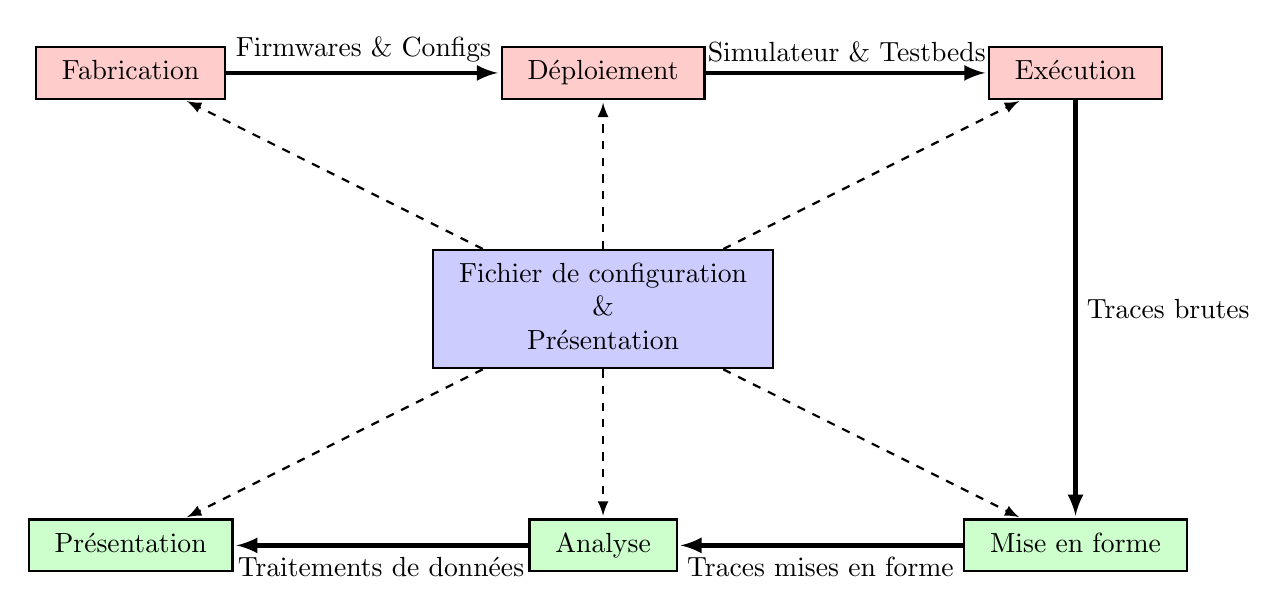
\begin{tikzpicture}[->,>=latex,shorten >=1pt,auto,node distance=3cm,
    thick,
    main node/.style={fill=blue!20,draw},
    pre node/.style={fill=red!20,draw},
    post node/.style={fill=green!20,draw}
    ]

    \node[pre node] (make) at (0, 3) {\begin{tabular}{c}Fabrication\end{tabular}};
    \node[pre node] (deploy) at (6, 3) {\begin{tabular}{c}Déploiement\end{tabular}};
    \node[pre node] (run) at (12, 3) {\begin{tabular}{c}Exécution\end{tabular}};

    \node[post node] (parse) at (12, -3) {\begin{tabular}{c}Mise en forme\end{tabular}};
    \node[post node] (analyze) at (6, -3) {\begin{tabular}{c}Analyse\end{tabular}};
    \node[post node] (plot) at (0, -3) {\begin{tabular}{c}Présentation\end{tabular}};
    
    % \node[main node] (analyze) at (12,0) {\begin{tabular}{c}Analyse\end{tabular}};

    \node[main node] (ipython) at (6,0) {\begin{tabular}{c}Fichier de configuration\\ \& \\Présentation\end{tabular}};

    \path
       (make) edge[ultra thick] node[above] {Firmwares \& Configs} (deploy) 
       (deploy) edge[ultra thick] node[above]  {Simulateur \& Testbeds} (run)
       (run) edge[ultra thick] node[right] {Traces brutes} (parse) 
       (parse) edge[ultra thick] node[below] {Traces mises en forme} (analyze)
       (analyze) edge[ultra thick] node[below] {Traitements de données} (plot)

  (ipython) edge[dashed] (make)
  (ipython) edge[dashed] (deploy)
  (ipython) edge[dashed] (run)
  (ipython) edge[dashed] (parse)
  (ipython) edge[dashed] (analyze)
  (ipython) edge[dashed] (plot)
  ;
  \end{tikzpicture}
  \caption{Découpage des étapes d'une expérience par Makesense}
  \label{makesense:fig:schema}
\end{figure}

Une expérience peut être découpée en différentes étapes qui se suivent dans un ordre logique.
Le schéma~\ref{makesense:fig:schema} illustre comment les différentes étapes d'une expérience typique à propos des \ac{LLN}s se suivent.

La \emph{fabrication} produit tous les binaires et fichiers de configurations initiaux qui sont nécessaires à une expérience.
La phase de \emph{déploiement} déplace ces fichiers sur les bonnes machines.
La phase d'\emph{exécution} lance et maintient les processus nécessaires à une expérience et de produire les traces brutes qui correspondent aux grandeurs mesurées.
La phase de \emph{mise en forme} ``nettoie'' des traces brutes afin de les rendre plus simples à analyser et exploiter.
La phase d'\emph{analyse} traite ces données mises en forme afin de produire des analyses qualitatives et quantitatives sur les phénomènes observés.
Enfin, la phase de \emph{présentation} fournit les représentations graphiques qui seront le plus souvent mises dans des articles ou partager avec d'autres collaborateurs.

Chacune des cellules de code utilisée peut être précédée ou suivie de plusieurs cellules de textes enrichis pour décrire ce qu'elle contient ou apporter des précisions sur son fonctionnement.
Les résultats intermédiaires des cellules de code peuvent être conservés dans le contexte commun à toutes les cellules du notebook ce qui permet de réutiliser des résultats et au besoin d'ajouter une nouvelle cellule pour explorer une nouvelle idée.

\subsubsection{Expérience séquentielle et script d'exécution}
\label{makesense:sequentiel}

Comme vu dans la section~\ref{makesense:related_automatisation}, il est nécessaire d'utiliser un outil de gestion de dépendance de tâches pour s'assurer que toutes les dépendances d'une tâche sont exécutées.
Or comme l'illustre le schéma~\ref{cache:fig:schema}, une expérience typique est bâtie autour d'un succession séquentielle d'étapes.
Ainsi l'organisation du code d'un notebook en succession d'étapes est acceptable pour ce type d'expérience rendant les outils génériques de gestion de dépendances de tâches tel que \texttt{make} non nécessaire par rapport aux besoins.

Il est donc possible de mettre chacune des étapes d'une expérience dans une cellule spécifique ce qui permet de rendre une expérience modulaire, car on peut obtenir le résultat d'une étape donnée en exécutant seulement une fois ses dépendances et en conservant les résultats intermédiaires.
Ce découpage permet de ne pas imposer de formalismes lourds sur une expérience et permet d'avoir une grande flexibilité sur son organisation.

Ce flot séquentiel est également adapté pour fournir un programme validant une par une toutes les étapes pour aboutir à la production des résultats.
Ce programme séquentiel est obtenu par l'extraction des cellules de code du notebook qui fournissent un programme pouvant reproduire l'exécution complète de l'expérience.
Ainsi il est possible de tirer parti de ce programme pour tester de manière systématique que l'expérience fonctionne d'une révision à l'autre.

\subsection{Garantie de reproductibilité d'une expérience}

Une expérience doit évoluer au cours du temps afin de corriger ses erreurs et obtenir de nouveaux résultats.
Cependant cette évolution ne doit pas se faire au détriment de la stabilité des résultats précédemment obtenus, car un processus expérimental se construit sur des acquis pour ensuite les étendre.

Un processus de développement logiciel efficace doit garantir une conservation des différentes révisions afin de revenir en arrière si une erreur est introduite ou bien de gérer les révisions concurrentes de plusieurs contributeurs.
Ainsi des logiciels spécifiques ont été introduits pour tenir compte de ces révisions et les gérer efficacement.
Les gestionnaires de versions sont aujourd'hui une fondation du développement logiciel et sont largement utilisés~\cite{o2009making}.

Makesense utilise un gestionnaire de révisions afin de garder en mémoire les différentes révisions d'un notebook.
L'observation des différences entre les différentes révisions est importante pour comprendre comment chaque révision modifie un notebook donné.
\texttt{git} est le gestionnaire de révision de référence de Makesense car il permet de disposer depuis la plateformes Github d'un rendu automatique du notebook pour toutes ces révisions successives~\cite{loeliger2012version,dabbish2012social}.
Cependant, Makesense est complètement agnostique sur le gestionnaire de version utilisé et ne l'utilise que pour mettre en place des mécanismes d'intégration continue.

\subsubsection{Intégration continue}
\label{makesense:ci}

L'obsolescence d'un programme peut arriver quand aucun test n'est présent pour s'assurer qu'il fonctionne ou non au cours de ses révisions successives.
Pour éviter cette obsolescence, il est nécessaire d'utiliser un processus systématique qui va vérifier à chaque révision que les résultats précédemment obtenus sont toujours valides.
Comme vu dans la section~\ref{makesense:sequentiel}, un notebook peut être transformé en script qui va exécuter séquentiellement une expérience pour en fournir les résultats.

L'\emph{intégration continue} est un ensemble de pratiques utilisées en production de logiciel qui consiste à vérifier que chaque modification apportée à un programme ne modifie pas son fonctionnement et qu'aucune régression fonctionnelle n'est introduite~\cite{duvall2007continuous}.
Son principal but est de détecter les problèmes et les erreurs afin de les corriger au plus tôt et de raccourcir les cycles de développement.
Massivement pratiquée par les acteurs principaux du développement logiciel elle a engendré de nouveaux courants et méthodologies logicielles comme que le \ac{TDD}~\cite{beck2003test} qui ont prouvé leur efficacité pour réduire le nombre d'erreurs au cours du développement d'un logiciel~\cite{maximilien2003assessing}. 

L'intégration continue est déclenchée quand une proposition de changement \footnote{``pull request'' dans le cas où on utilise \texttt{git}.} est poussée vers le dépôt gérant les versions du notebook.
Une copie de la version révisée est envoyée sur le serveur d'intégration continue qui va créer l'environnement pour le notebook, extraire les cellules de code puis exécuter le programme engendré.
Une fois l'exécution terminée et sans erreur, on a la garantie que le changement n'a pas engendré une erreur sur un résultat existant~\footnote{On parle de test de non-régression.}.
Une fois que le résultat est conforme aux tests demandés, il peut être intégré à la branche principale de développement et le processus se répète pour tout nouveau changement proposé.

Cette méthodologie de développement logicielle combinée a un script extrait d'un notebook permet de garantir que l'expérience contenue reste reproductible.

L'intégration continue dans le cas d'expérience sur un \ac{LLN} garantit que toutes les dépendances requises pour créer une expérience, l'exécuter et exploiter les résultats sont documentées, installées avec une intégration testée et fonctionnelle.

Makesense versionne l'évolution du notebook contenant l'expérience de cette section en utilisant \texttt{git} et en l'hébergeant sur Github.
Lorsqu'une nouvelle révision est proposée (pour ajouter une étape, changer une variable), une proposition de révision est envoyée pour être relue par les propriétaires du dépôt hébergeant le notebook.
Lorsque la proposition de révision est initiée, une copie de la version modifiée est envoyée vers le serveur d'intégration continue qui déterminera si cette révision est acceptable.
Cette vérification est obtenue en procédant à l'extraction des cellules de code du notebook et l'exécution du script obtenu.
Une fois cette vérification faite, la révision peut être intégrée au dépôt du notebook et ce cycle se répète à chaque révision proposée.

\subsection{Approvisionnement d'une expérience}

L'approvisionnement d'une expérience consiste à préparer tous les fichiers et systèmes nécessaires au déroulement d'une expérience.
Les expériences sur \ac{LLN}s mettent en jeu des nœuds ayant des configurations spécifiques par exemple sur la fréquence d'envoi d'un message.
Configurer chaque nœud de manière ad hoc n'est pas envisageable à mesure que le nombre de nœuds et les paramètres mis en jeu grandissent.
Afin de réaliser des expériences à grande échelle, le langage utilisé pour décrire l'expérience doit être suffisamment souple et expressif pour initialiser facilement chaque nœud à partir d'un modèle de base.

La mise en œuvre de cette phase de configuration dans Makesense consiste à créer à partir de gabarits de base (appelé ``template'' en anglais), les fichiers qui seront utilisés et compilés au cours de l'expérience.
Chaque fichier nécessaire à l'expérience va être construit à partir d'un gabarit de base qui va être remplis par un moteur de gabarit (aussi appelé ``templating engine'' en anglais) avec les variables qui lui sont propres.
Ce type de pratique par gabarit a déjà été utilisé et validé à large échelle dans le contexte de configuration de serveurs et de configuration de serveurs~\cite{hochstein2014ansible} ainsi son utilisation dans le contexte de la configuration des nœuds capteurs se rapproche de cette utilisation.

Dans le cas typique des expériences portant sur un \ac{LLN}, cette étape de préparation compile les systèmes d'exploitation pour les nœuds contraints et produit tous les fichiers de configuration nécessaires à la simulation.
Dans le cas du binaire exécuté par les nœuds, il est obtenu pour différentes architectures~\footnote{L'émulation dans COOJA s'effectue sur l'architecture MSP430 et les nœuds IoT-lab utilisent l'architecture ARM dans le cas des Cortex M3.}.

Une simulation dans Cooja requiert la création d'un fichier principal qui va être utilisé pour placer les nœuds, les démarrer avec le bon binaire, interagir avec eux, configurer leur portée de transmission ou la graine des générateurs de nombres aléatoires utilisée pendant la simulation.
Ainsi, Makesense fournit un gabarit de fichier de configuration qui est peuplé dynamiquement et enregistré pour être utilisé ensuite.
Le rendu de la topologie est fait automatiquement et les binaires sont compilés correctement avec leurs variables propres et sont affectés aux nœuds correspondants dans le fichier de configuration de la simulation.

\subsection{Déploiement - Exécution et récupération des traces}
\label{automation:deploy_execute_move}

L'objectif des phases de déploiement, d'exécution et de déplacement des traces est de produire une exécution de l'expérience visée et de déplacer toutes les traces pertinentes de cette expérience vers une destination spécifique pour y être analysées.
Cette phase est délicate car elle met en jeu de nombreux processus.
Elle est documentée et automatisée par Makesense afin de fournir autant que faire se peut une reproductibilité de l'expérience qu'elle se passe dans un simulateur ou sur plateforme.

\subsubsection{Déploiement}

La phase de déploiement déplace les fichiers produits lors de l'approvisionnement vers la machine où ils seront utilisés.

Makesense déploie une expérience vers un serveur ou une plateforme en utilisant les \ac{API} ou un accès à distance automatisable.
Ainsi toute plateforme ou machine utilisant un accès à distance automatisable est utilisable par Makesense.

Dans le cas de l'exécution d'une simulation sur la même machine, ce déploiement correspond à une simple copie des fichiers pertinents.
Cependant, dans le cas de simulations devant être exécutées sur des grilles de calcul, il est nécessaire mémoriser sur quels serveurs l'expérience a été déployée afin d'en récupérer les résultats.

L'utilisation d'un testbed permet de confirmer les résultats d'un simulateur par une exécution de l'expérience sur des nœuds physiques.
Dans le cas de testbed mutualisées, il faut gérer des réservations de nœuds qui sont potentiellement accessibles par tous les utilisateurs de la plateforme et qui peuvent également tomber en panne.
Ainsi il est nécessaire de maintenir dynamiquement une table de correspondance entre les  nœuds réservés et le code qui y est exécuté.
Automatiser ce processus de déploiement permet de choisir dynamiquement les nœuds mis en jeu lors d'une expérience (par exemple les moins chargés, les mieux placés, etc.).

Plusieurs testbeds publics tels que Indriya~\cite{doddavenkatappa2011indriya} ou bien IoT-lab~\cite{fleury2015fit} sont disponibles afin d'exécuter une expérience sur des nœuds physiques.
Makesense supporte IoT-lab par l'utilisation de la bibliothèque officielle pour réserver et démarrer des expériences.
La plateforme IoT-lab a été choisie en raison de la variété des nœuds physiques proposés, du support des systèmes d'exploitation de référence sur ses nœuds et de son processus de réservation et d'accès à distance facilement automatisable.
IoT-lab met à disposition de ses utilisateurs, sur plusieurs sites physiques ayant la même interface, des nœuds physiques supportant \ieee{} représentatifs de nœuds capteurs.
Pour fonctionner, IoT-lab utilise, entre autre, des serveurs (nommés ``front-end'') sur lesquels des utilisateurs peuvent se connecter par \ac{SSH} et lancer des commandes visant à interagir avec les nœuds physiques.
Makesense utilise la bibliothèque officielle d'IoT-lab afin de faire les réservations et d'envoyer les binaires utilisés par les nœuds physiques.
Dans le cas où d'autres programmes doivent être déployés sur les serveurs d'IoT-lab, Makesense y accède par \ac{SSH} afin d'y envoyer les fichiers requis.

\subsubsection{Exécution}

Lors de l'exécution d'une expérience, il est courant d'avoir plusieurs processus lancés en parallèle pour effectuer différentes fonctions.
Parmi ces processus, certains vont par exemple, générer les traces brutes qui vont être utilisées par la suite pour analyser le déroulement d'une expérience.

Ces processus sont parfois nombreux, s'exécutent avec différents privilèges, sur différentes machines et dans un certain ordre.
En outre, il faut s'assurer qu'une fois lancés, ces processus continuent de fonctionner correctement durant toute l'expérience.
Gérer manuellement ces processus comporte plusieurs risques, d'une part, il est possible d'en oublier un ou bien de les lancer dans le désordre causant l'échec de l'expérience si ces processus sont critiques.
De plus, dans le cas où les expériences durent longtemps, il est nécessaire de maintenir une surveillance continue de l'expérience et de chacun de ces processus.

Makesense permet de documenter le lancement de ces processus en les mettant dans des objets qui sont gérés de manière automatisée.
Ainsi les processus sont systématiquement lancés et dans le même ordre permettant d'éviter les écueils d'un lancement manuel.
D'autre part, il est possible d'avoir au cours de l'exécution le statut d'un processus et le relancer le cas échéant.

\subsubsection{Récupération des traces}

Une expérience, qu'elle se produise dans un simulateur ou sur nœuds physiques, génère de nombreuses données brutes comme des fichiers \ac{PCAP}~\cite{mccanne1989libpcap} qui décrivent le trafic réseau ou encore des journaux d’événements (appelés ``logs'' en anglais).

Afin de simplifier les traitements, il est pratique de rassembler toutes ces traces sur une seule machine qui va être utilisée pour traiter ces données.
Ainsi il est nécessaire d’agréger les différents fichiers de données en provenance de sources multiples vers une seule destination.
Automatiser ces traitements permet de garantir qu'aucun de ces fichiers n'est oublié, de documenter ceux qui seront traités et ceux non pertinents qui seront évités.

Makesense peut déplacer toutes les traces brutes depuis une machine donnée (par exemple une grille de calcul ou un front end IoT-lab) vers une autre (par exemple une station de travail locale ou un ordinateur portable).

Dans le cas d'une expérience sur IoT-lab, l'identifiant d'expérience qui est donné lors de la réservation d'une expérience permet d'obtenir l'adresse du dossier contenant les résultats sur le serveur front end.
Ainsi Makesense récupère les traces dynamiquement en fonction de cet identifiant et sur l'ensemble des fichiers pertinents ce qui est plus efficace qu'une récupération manuelle de chaque fichier individuel.

\subsection{Exploitation des résultats}

L'exploitation de résultats est la phase permettant d'étudier de manière quantitative et qualitative une expérience en utilisant ses traces.
Les étapes que cette phase comporte étant dissociées des contraintes des \ac{LLN}s, tous les traitements peuvent utiliser des outils généraux et communs à de nombreux champs de recherche scientifique.
Cette phase est complètement automatisable et déterministe, car elle applique des traitements fixes à des traces fournies en amont.
L'objectif de cette phase consiste d'une part à décoder toutes les traces brutes pour en extraire les informations les plus pertinentes et d'autre part à fournir des données pour une interprétation quantitative et qualitative de l'expérience.

\begin{figure}[ht]
\centering
\begin{tikzpicture}[->,>=latex,shorten >=1pt, thick,main node/.style={fill=blue!20,draw}]

  \node[main node] (parse) {\begin{tabular}{c}Mise en forme\end{tabular}};

  \node[main node, below left=of parse] (pcap) {\begin{tabular}{c}PCAP\end{tabular}};
  \node[main node, above left=of parse] (logs) {\begin{tabular}{c}Logs\end{tabular}};

  \node[main node, right=of parse] (good_data) {\begin{tabular}{c}Données mises en forme\end{tabular}};
  \node[main node, above=of good_data] (analysis) {\begin{tabular}{c}Analyse des données\end{tabular}};

  \node[main node, below=of good_data] (csv) {\begin{tabular}{c}Export vers CSV\end{tabular}};


  \path
       (pcap) edge[->] (parse.south west) 
       (logs) edge[->] (parse.north west) 
       (parse) edge[->] (good_data) 
       (good_data)  edge[->] (analysis)
       (good_data) edge[->] (csv) 
  ;

\end{tikzpicture}
\caption{Transformation des traces brutes vers des formats de données standards}
\label{makesense:fig:data_clean}
\end{figure}

La Figure~\ref{makesense:fig:data_clean} illustre l'approche choisie par Makesense.
Le processus de transformation vise à aboutir à des données mises en forme qui seront exploitées directement lors de la phase d'analyse et qui peuvent être exportées au besoin vers un format standard pour être partagées.

\subsubsection{Mise en forme de traces brutes}

Les traces brutes sont de nature hétérogène, une première étape de la phase de traitement consiste à transformer ces résultats bruts vers des fichiers plus exploitables et homogènes.
L'objectif de cette approche est de distinguer la phase de décodage d'une trace de son interprétation.

Dans le cas d'une expérience portant sur les \ac{LLN}s, il s'agit par exemple de transformer les fichiers \ac{PCAP} et les multiples journaux textes représentant les événements qui se sont produits par des transformations pour obtenir des traces plus exploitables.

Une conversion ad hoc aurait du mal à fonctionner pour un grand nombre de fichiers et de traitements différents.
En outre, documenter les traitements effectués permet d'avoir une documentation sur les formats de documents obtenus afin d'éviter les traitements ad hoc.
Enfin, transformer les données vers un format standard comme \ac{CSV} permet de les importer dans de nombreux outils plus facilement notamment dans le cas de données tabulaires.
Ainsi les mêmes traces peuvent être réutilisées pour des expériences voulant explorer différentes conclusions autour de données communes.

Makesense implémente ces transformations en utilisant des bibliothèques logicielles dédiées aux traitements de données tabulaires.
L'objectif est d'appliquer à chaque élément d'une trace toutes les transformations nécessaires (renommage, normalisation, etc.) afin d'obtenir des tableaux et d'autres structures de données facilement exportables et manipulables.

\subsubsection{Analyse des résultats}

La phase d'analyse de résultats traite les données mises en forme afin de permettre leur interprétation et de fournir des résultats qualitatifs ou quantitatifs sur une expérience.
Elle doit être facilitée par des itérations aussi courtes que possible pour tester de nouvelles hypothèses afin de diminuer le temps nécessaire pour confirmer ou infirmer une hypothèse sur une expérience.

Makesense met à profit des bibliothèques logicielles scientifiques afin d'effectuer ces traitements~\cite{mckinney2012python}.
Les données mises en forme sont chargées dans des structures de données tabulaires où il est facile de les filtrer sur certains critères et de les agréger par différentes fonctions (une somme, un comptage, etc.).
Le rendu de ces données peut être fait sous forme graphique avec des graphes qui illustrent les phénomènes observés.

Dans le cas d'expériences sur les \ac{LLN}s, il est par exemple nécessaire d'exploiter les données disponibles dans les traces de trafic réseau en utilisant un dissecteur de paquets comme Wireshark~\cite{tshark}.
Ces traces présentées dans le notebook sous la forme de tableau représentent pour chaque paquet les attributs trouvés par le dissecteur (source, destination, protocole, taille, etc.).
Ainsi pour analyser la répartition de protocoles réseau, il suffit d'effectuer une requête similaire sémantiquement à une requête faite sur une base de données relationnelle classique~\cite{mckinney2012python}.
Ce formalisme permet une grande expressivité sur les données recueillies et permet de s'abstraire des représentations concrètes des données dans les fichiers pour se concentrer sur ce qu'elles représentent.
Ces données une fois trouvées peuvent être représentées par des visualisations et des graphes par des outils graphiques~\cite{Hunter:2007}.

Un autre exemple consiste à avoir une représentation graphique de la topologie du réseau formée par les nœuds directement dans le notebook.
Cela permet d'identifier rapidement les dysmétries et les nœuds importants pour la connexité du graphe.
De plus, une fois cette représentation du \ac{DODAG} \ac{RPL} disponible, il est possible de calculer les plus courts chemins entre un nœud et la racine du \ac{DODAG} afin d'obtenir la profondeur d'un nœud.

Ces fonctionnalités de groupement d'informations permettent d'exprimer de manière concise des traitements sur les données pour en extraire les informations utiles.

\section{Conclusion} 
\label{makesense:conclusion}

Ce chapitre montre qu'afin de permettre le partage et la reproductibilité d'une expérience, sa documentation et son automatisation jouent un rôle clé.
Ce processus est assez systématique et dépasse largement le contexte des \ac{LLN}s, ainsi des outils et des méthodologies communes peuvent émerger pour proposer des solutions à des problèmes communs.

Makesense est une réponse possible et se veut générique en utilisant des bibliothèques généralistes et répandues dans de multiples domaines de développement logiciel scientifique ou général.
Makesense propose de documenter et d'automatiser une expérience pour \ac{LLN} transcrite dans un notebook pour s'assurer de sa reproductibilité.
La reproductibilité d'une expérience est une nécessité des projets de recherche.
La réduction de la complexité de la mise en place d'une expérience permet d’accélérer une étude et d'augmenter son impact en facilitant sa vérification et son partage.
À cette fin, Makesense est disponible sous licence Apache sur Github~\footnote{\href{https://github.com/sieben/makesense}{https://github.com/sieben/makesense}} et une démonstration du déroulement d'une expérience est également disponible~\footnote{\href{https://travis-ci.org/sieben/makesense}{https://travis-ci.org/sieben/makesense}}.
Étant diffusé sous licence libre, il est difficile d'estimer son utilisation globale, cependant la version initiale disponible sur PyPI a été téléchargée plus de 1000 fois.

Makesense a été utilisé afin de réaliser les expériences décrites dans les chapitres suivants et pourrait être mis à profit afin d'avoir une solution permettant d'avoir une intégration complète d'une expérience dans le but de la diffuser.

Makesense ne gère pas pour le moment les erreurs à la volée qui peuvent subvenir lors d'une expérience.
Or dans le cas de tests sur nœuds réels, ces erreurs peuvent être nombreuses par exemple dans le cas d'erreurs de flashage ou de panne d'un nœud.
Il est alors nécessaire de redémarrer le nœud brutalement et cela ne garantit pas que le problème n'arrivera pas de nouveau.

Avoir une gestion plus fine et réactive des processus permettrait de prendre des décisions plus raisonnées dans le but d'avoir un environnement plus contrôlable.
Cependant cette tâche est délicate, car les pannes et problèmes qui peuvent subvenir sont très hétérogènes et il est difficile de prendre des décisions automatiques dans ce genre de cas notamment dans le cas de testbeds mutualisées ou le contrôle de l'environnement et de ses interférences n'est pas facilement réalisable.

Une autre fonctionnalité pourrait être la gestion de points d'étapes (``checkpoint'' en anglais) dans une expérience qui permettrait de sauvegarder l'intégralité du contexte d'une expérience à un instant donné.
Cette fonctionnalité serait particulièrement utile pour effectuer des analyses post mortem d'un système tombé en panne.

Les méthodologies modernes de développement logiciel peuvent influencer les méthodologies expérimentales scientifiques notamment en informatique où de nombreux outils sont communs.
La création de communautés autour des différents outils logiciels utilisés par la communauté scientifique facilite les échanges et la diffusion de nouvelles méthodes plus efficaces pour résoudre les problèmes communs.
Makesense illustre comment intégrer efficacement ces technologies afin d'aider les expériences sur les \ac{LLN}s à être plus reproductibles.
Ce framework est mis à profit dans les expériences des chapitres~\ref{cache} et~\ref{supervision}.

\section*{Publications et invitations relatives à Makesense}

\begin{itemize}
  \item Rémy Leone, Jeremie Leguay, Paolo Medagliani, Claude Chaudet, et~al.
\newblock Makesense: Managing reproducible wsns experiments.
\newblock {\em Fifth Workshop on Real-World Wireless Sensor Networks}, 2013.

  \item Rémy Léone, Jérémie Leguay, Paolo Medagliani, and Claude
  Chaudet.
\newblock Demo abstract: Makesense—managing reproducible wsns experiments.
\newblock In {\em Real-World Wireless Sensor Networks}, pages 65--71. Springer,
  2014.

  \item Rémy Léone, Jérémie Leguay, Paolo Medagliani, and Claude
  Chaudet.
\newblock Demo Abstract: Automating WSN experiments and simulations.
\newblock In {\em EWSN}, 2015.

  \item Invitation au colloque R4: Retour d'expéRiences sur la Recherche Reproductible.
  \newblock Le Studium - Centre International Universitaire pour la Recherche - Orléans
  \newblock 3 et 4 décembre 2015 

\end{itemize}
